\section{Introduction}
\begin{frame}{\VideoName}
    \tableofcontents[currentsection]
\end{frame}

\begin{frame}{Classical power analysis attack methods}
    \begin{itemize}
        \item \textit{Simple power analysis (SPA)} assumes the attacker has access to only one or a few measurements corresponding to some fixed inputs.
        \item \textit{Differential power analysis (DPA)} assumes the attacker can take measurements for a potentially unlimited number of different inputs.
       \item We will see
       \begin{itemize}
           \item SPA on RSA
           \item DPA on symmetric block ciphers (example: PRESENT)
       \end{itemize}
    \end{itemize}
\end{frame}

\begin{frame}{RSA}
\begin{definition}[RSA]
Let $n=pq$, where $p,q$ are distinct prime numbers.
Let $\mathcal{P}=\mathcal{C}=\ZZ_n$, $\mathcal{K}=\ZZ_{\varphi(n)}^*-\Set{1}$.
For any $e\in \mathcal{K}$, define encryption
\[
    E_e:\ZZ_n\to\ZZ_n,\quad m\mapsto m^e\mo n,
\]
and the corresponding decryption
\[
    D_d:\ZZ_n\to\ZZ_n,\quad c\mapsto c^d\mo n,
\]
where $de\mo\varphi(n)=1$.
The cryptosystem $(\mathcal{P},\mathcal{C},\mathcal{K},\mathcal{E},\mathcal{D})$, where $\mathcal{E}=\Set{E_e:e\in\mathcal{K}}$, $\mathcal{D}=\Set{D_d:d\in\mathcal{K}}$, is called \textit{RSA}.
\end{definition}
\begin{itemize}
    \item $\varphi(n)=(p-1)(q-1)$
    \item Public key: $n,e$, RSA modulus, encryption exponent
    \item Private key: $d$, decryption exponent
\end{itemize}
\end{frame}

\begin{frame}{Remark}
    \begin{itemize}
        \item Since $\varphi(n)=(p-1)(q-1)$ is even and $\gcd(d,\varphi(n))=1$, $d$ is odd.
         \item In particular LSB of $d$ is $=1$.
    \end{itemize}
\end{frame}

\begin{frame}{Square and multiply algorithm}
    \begin{itemize}
        \item Let $n\geq2$ be an integer, $d\in\ZZ_{\varphi(n)}^{*}$, $a\in\ZZ_n$
        \item Binary representation of $d=d_{\ell_d-1}\dots d_2d_1d_0$, where $d_i=0,1$ and
\[
d=\sum_{i=0}^{\ell_d-1}d_i2^i,
\]
\item Then we have
\[
a^d=a^{\sum_{i=0}^{\ell_d-1}d_i2^i}=\prod_{i=0}^{\ell_d-1}(a^{2^i})^{d_i}=\prod_{0\leq i<\ell_d,d_i=1}a^{2^i}.
\]
Thus, to compute $a^d\mo n$, we can 
\begin{itemize}
    \item first compute $a^{2^i}$ for $0\leq i<\ell_d$
    \item then $a^d$ is a product of $a^{2^i}$ for which $d_i=1$
\end{itemize}
    \end{itemize}
\end{frame}

\begin{frame}{Left-to-right square and multiply algorithm}
    \begin{algorithm}[H]
\KwIn{$n,\ a,\ d$\tcp{$n\in\ZZ, n\geq2$; $a\in\ZZ_n$; $d\in\ZZ_{\varphi(n)}$}}
\KwOut{$a^d\mo n$}
$t = 1$\\
	\For{$i=\ell_d-1$, $i\geq0$, $i--$}
 	{
  	$t=t*t\mo n$\\
 	\tcp{$i$th bit of $d$ is $1$}
  		\If{$d_i=1$}{
  		$t = a*t\mo n$
  		}
  	}
  	\Return a
\caption{Left-to-right square and multiply algorithm for computing modular exponentiation.}
\end{algorithm}
\end{frame}

\section{SPA on RSA}
\begin{frame}{\VideoName}
    \tableofcontents[currentsection]
\end{frame}

\begin{frame}{Left-to-right square and multiply algorithm}
For our experiment, we have set
        \[
        p=29,\quad q=41,\quad n=1189,\quad \varphi(n)=1120,\quad e=3,\quad d=747
        \]
{\small
\begin{algorithm}[H]
\KwIn{$a$\tcp{$a\in\ZZ_{1189}$}}
\KwOut{$a^{747}\mo 1189$}
$n=1189$\\
$dbin=[1,1,0,1,0,1,1,1,0,1]$\tcp{binary representation of $d=747$, $d_0=1$, $d_1=1$}
$\ell_d=\text{length of }dbin$\tcp{bit length of $d$}
$t = 1$\\
	\For{$i=\ell_d-1$, $i\geq0$, $i--$}
 	{
  	$t=t*t\mo n$\\
 	\tcp{$i$th bit of $d$ is $1$}
  		\If{$d_i=1$}{
  		$t = a*t\mo n$
  		}
  	}
  	\Return t
\caption{Left-to-right square and multiply algorithm for computing modular exponentiation with parameters from above.}
\end{algorithm}}
\end{frame}

\begin{frame}{Recall -- leakage is dependent on the operations being executed}
    \begin{figure}
    \centering
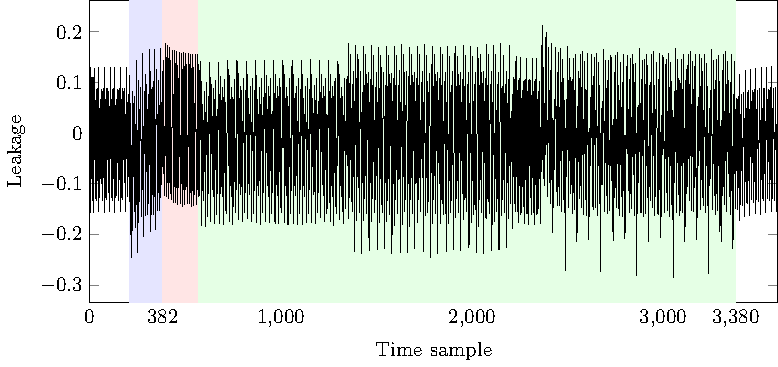
\includegraphics{fig/PRESENT_plot___one_round_average___highlighted_operations.pdf}
    \caption{The averaged trace for $5000$ traces from the \datafixone.
    The blue, pink, and green parts of the trace correspond to addRoundKey, sBoxLayer, and pLayer respectively.}
\end{figure}
\end{frame}

\begin{frame}{SPA on left-to-right square and multiply algorithm}
\begin{itemize}
    \item An SPA attack on the square and multiply algorithm exploits the leakage dependence on the performed operations -- we examine the traces to figure out if both square and multiplication are executed in one loop (the corresponding bit of $d$ is $1$) or not (the corresponding bit of $d$ is $0$).
    \item Following Kerckhoffs' principle, we assume the attacker has the knowledge of our algorithm except for line 2, which specifies the value of $d$
\end{itemize}
\begin{definition}[Kerckhoffs' principle]
The security of a cryptosystem should depend only on the secrecy of the key.
\end{definition}
\noindent
In other words, everything is public knowledge except for the secret key.
\end{frame}

\begin{frame}{SPA on left-to-right square and multiply algorithm}
\begin{figure}[H]
    \centering
    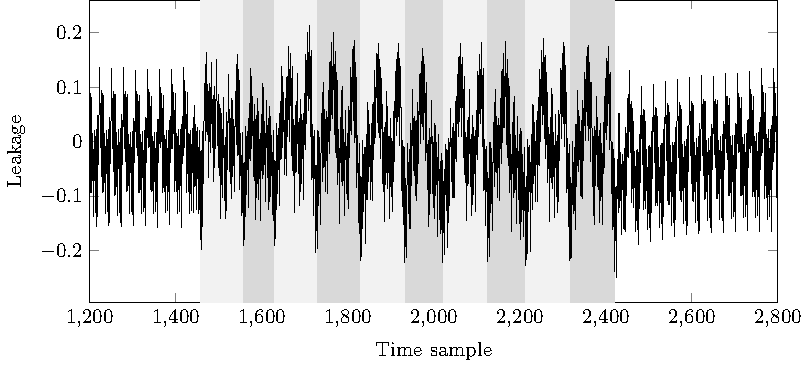
\includegraphics{fig/SPA_RSA_patterns.pdf}
    \caption{One trace.
    We can see $10$ similar patterns.}
\end{figure}
\end{frame}

\begin{frame}{What are those patterns}
\begin{columns}[T] % align columns
\begin{column}{.48\textwidth}
{
\setlength{\interspacetitleruled}{0pt}%
\setlength{\algotitleheightrule}{0pt}%
\begin{algorithm}[H]
	\KwIn{$a$\tcp{$a\in\ZZ_{1189}$}}
\KwOut{$a^{747}\mo 1189$}
$n=1189$\\
$dbin=[1,1,0,1,0,1,1,1,0,1]$\\
$\ell_d=\text{length of }dbin$\\
$t = 1$\\
	\For{$i=\ell_d-1$, $i\geq0$, $i--$\label{line:alg:SCA-RSA-implementation:loop}}
 	{
  	$t=t*t\mo n$\label{line:alg:SCA-RSA-implementation:tt}\\
  		\If{$d_i=1$}{
  		$t = a*t\mo n$\label{line:alg:SCA-RSA-implementation:at}
  		}
  	}
  	\Return t
\end{algorithm}
}
\end{column}%
\hfill%
\begin{column}{.57\textwidth}
We have two guesses
\begin{itemize}
    \item[Guess a] Each pattern corresponds to one modular operation (modular square from line~\ref{line:alg:SCA-RSA-implementation:tt} or modular multiplication from line~\ref{line:alg:SCA-RSA-implementation:at});
    \item[Guess b] Each pattern corresponds to one loop from line~\ref{line:alg:SCA-RSA-implementation:loop}.
\end{itemize}
\begin{itemize}
    \item S: modular square operation from line~\ref{line:alg:SCA-RSA-implementation:tt}
    \item M: modular multiplication from line~\ref{line:alg:SCA-RSA-implementation:at}.
    \item Loop in line~\ref{line:alg:SCA-RSA-implementation:loop} contains either one square operation (S) or one square followed by a multiplication operation (SM).
\end{itemize}
\[
\text{S} \longleftrightarrow d_i=0,\quad \text{SM} \longleftrightarrow d_i=1.
\]
\end{column}%
\end{columns}
\end{frame}

\begin{frame}{Two different patterns}
    \begin{figure}[H]
    \centering
    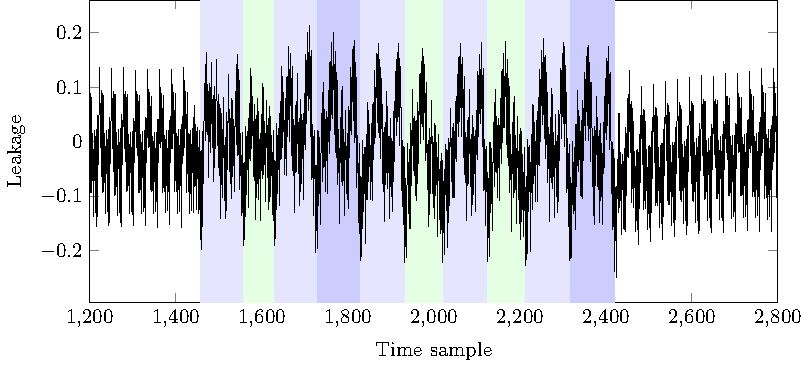
\includegraphics{fig/SPA_on_RSA_highlighted_peaks.pdf}
    \caption{Highlighted two types of patterns from the previous figure. One pattern with a single cluster of peaks (colored in green) and one with more than one cluster of peaks (colored in blue).}
\end{figure}
\end{frame}

\begin{frame}{Assume Guess a is correct}
   \begin{columns}[T] % align columns
\begin{column}{.48\textwidth}
{
\setlength{\interspacetitleruled}{0pt}%
\setlength{\algotitleheightrule}{0pt}%
\begin{algorithm}[H]
	\KwIn{$a$\tcp{$a\in\ZZ_{1189}$}}
\KwOut{$a^{747}\mo 1189$}
$n=1189$\\
$dbin=[1,1,0,1,0,1,1,1,0,1]$\\
$\ell_d=\text{length of }dbin$\\
$t = 1$\\
	\For{$i=\ell_d-1$, $i\geq0$, $i--$\label{line:alg:SCA-RSA-implementation:loop}}
 	{
  	$t=t*t\mo n$\label{line:alg:SCA-RSA-implementation:tt}\\
  		\If{$d_i=1$}{
  		$t = a*t\mo n$\label{line:alg:SCA-RSA-implementation:at}
  		}
  	}
  	\Return t
\end{algorithm}
}
\end{column}%
\hfill%
\begin{column}{.57\textwidth}
\begin{itemize}
    \item[Guess a] Each pattern corresponds to one modular operation (modular square from line~\ref{line:alg:SCA-RSA-implementation:tt} or modular multiplication from line~\ref{line:alg:SCA-RSA-implementation:at});
   \item There are two possibilities:
\begin{itemize}
    \item Green patterns $\rightarrow$ S; blue patterns $\rightarrow$ M 
    \item Green patterns $\rightarrow$ M; blue patterns $\rightarrow$ S 
\end{itemize}
    \item We know that $d_0=1$, hence the last blue-colored pattern does not represent S.
     \item The start of the computation will always be a modular square operation, which then indicates that the first blue-colored pattern corresponds to S.
     \item We have reached a contradiction
\end{itemize}
\end{column}%
\end{columns} 
\end{frame}

\begin{frame}{Assume Guess b is correct}
   \begin{columns}[T] % align columns
\begin{column}{.48\textwidth}
{
\setlength{\interspacetitleruled}{0pt}%
\setlength{\algotitleheightrule}{0pt}%
\begin{algorithm}[H]
	\KwIn{$a$\tcp{$a\in\ZZ_{1189}$}}
\KwOut{$a^{747}\mo 1189$}
$n=1189$\\
$dbin=[1,1,0,1,0,1,1,1,0,1]$\\
$\ell_d=\text{length of }dbin$\\
$t = 1$\\
	\For{$i=\ell_d-1$, $i\geq0$, $i--$\label{line:alg:SCA-RSA-implementation:loop}}
 	{
  	$t=t*t\mo n$\label{line:alg:SCA-RSA-implementation:tt}\\
  		\If{$d_i=1$}{
  		$t = a*t\mo n$\label{line:alg:SCA-RSA-implementation:at}
  		}
  	}
  	\Return t
\end{algorithm}
}
\end{column}%
\hfill%
\begin{column}{.57\textwidth}
\begin{itemize}
   \item[Guess b] Each pattern corresponds to one loop from line~\ref{line:alg:SCA-RSA-implementation:loop}.
\item There are two possibilities:
\begin{itemize}
    \item Green patterns $\rightarrow$ $d_i=0$; blue patterns $\rightarrow$ $d_i=1$ 
    \item Green patterns $\rightarrow$ $d_i=1$; blue patterns $\rightarrow$ $d_i=0$ 
\end{itemize}
    \item We know that $d_0=1$, hence the last blue-colored pattern does not represent $d_i=0$.
    \item Green patterns $\rightarrow$ $d_i=0$; blue patterns $\rightarrow$ $d_i=1$ 
\end{itemize}
\end{column}%
\end{columns} 
\end{frame}

\begin{frame}{The secret key}
    \begin{figure}[H]
    \centering
    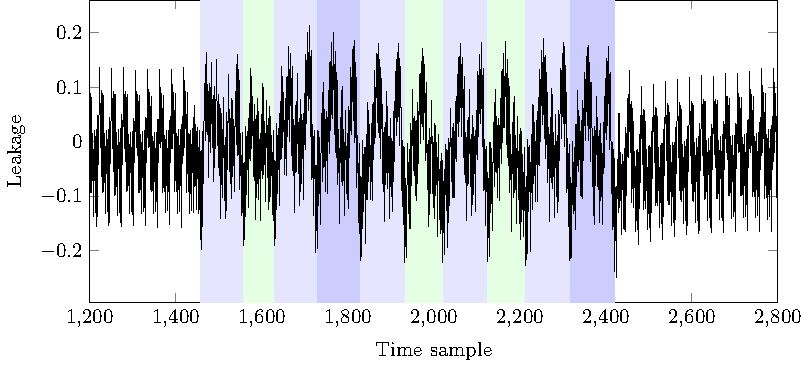
\includegraphics[width=0.8\textwidth]{fig/SPA_on_RSA_highlighted_peaks.pdf}
    % \caption{Green patterns $\rightarrow$ $d_i=0$; blue patterns $\rightarrow$ $d_i=1$}
\end{figure}
We can then read out the value of bits $d_i$ ($i=\ell_d-1,\dots,0,1$):
\[
1\quad 0\quad 1\quad 1\quad 1\quad 0\quad 1\quad 0\quad 1\quad 1.
\]
Finally, we recover the secret key
\[
d=1011101011_2=747.
\]
\end{frame}

\begin{frame}{The second pattern}
\begin{figure}[H]
    \centering
    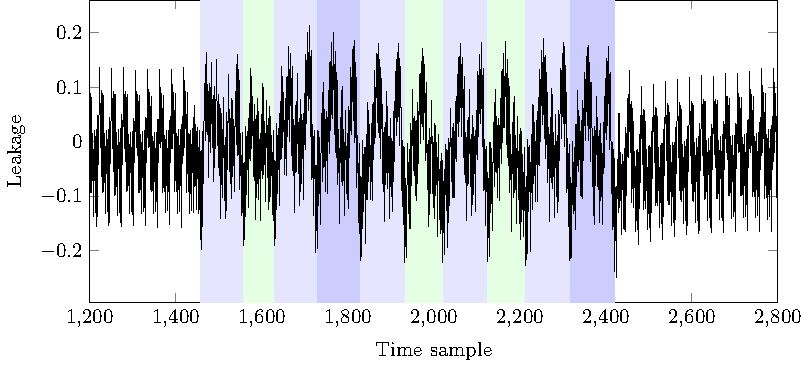
\includegraphics[width=0.8\textwidth]{fig/SPA_on_RSA_highlighted_peaks.pdf}
    % \caption{Green patterns $\rightarrow$ $d_i=0$; blue patterns $\rightarrow$ $d_i=1$}
\end{figure}
    \begin{itemize}
        \item It is not clear whether the second pattern should be green or blue
        \item Shorter than blue patterns
        \item In reality, brute force
    \end{itemize}
\end{frame}

\begin{frame}{Remark}
    \begin{itemize}
        \item A similar SPA attack can also be applied to the right-to-left square and multiply algorithm.
        \item The attack can be carried out during either the decryption of RSA or the signature signing procedure of RSA signatures.
    \end{itemize}
\end{frame}